% https://tex.stackexchange.com/a/325472
\documentclass[11pt]{beamer}
\usetheme{default}
\usepackage[utf8]{inputenc}
\usepackage[T1]{fontenc}
\usepackage{tikz,pgfplots}
\usepackage{xcolor}
\usepackage{xstring}
\pgfplotsset{compat=newest}

\newcommand*{\diff}{}% Ensure it is not already defined
\newcommand*{\clr}{}% Ensure it is not already defined

\author{Me}
\title{Stuff}
\subtitle{More stuff}
\logo{Logo}
\institute{School}
\date{Today}
\subject{Math stuff}
\setbeamercovered{transparent}

\begin{document}

    \begin{frame}[fragile]
        \frametitle{Multicolor chart}

        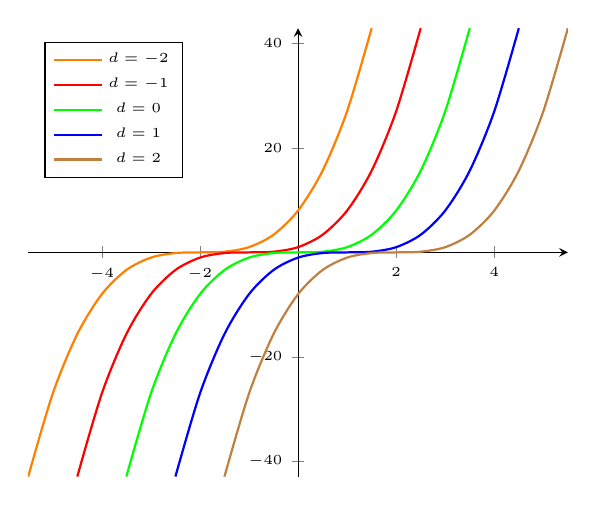
\begin{tikzpicture}[font=\tiny]
        \begin{axis}[
        axis x line=center,
        axis y line=center,
        restrict y to domain=-50:50,
        legend entries={$d=-2$,$d=-1$,$d=0$,$d=1$,$d=2$},legend pos=north west]%or north west, ... ,outer north east
        ]
        \pgfplotsinvokeforeach{-2/orange, -1/red, 0/green, 1/blue, 2/brown}
        {
            \StrBefore{#1}{/}[\diff]%
            \StrBehind{#1}{/}[\clr]%
            \edef\AddPlot{\noexpand\addplot[thick,smooth,color=\clr,domain=-6:6
                ] {(x-\diff)^3};}%
            \AddPlot
        }
        \end{axis}
        \end{tikzpicture}
\end{frame}
\end{document}
